\documentclass[../main.tex]{subfiles}
\graphicspath{{\subfix{../Images/}}}
\begin{document}

%\section{GB-CACHE} \label{gbcache}

In parallel with vision-based detection, this research employs the LiDAR-centric method GB-CACHE to represent the class of geometry-driven clustering and segmentation algorithms.
% optimized for sparse maritime environments.
Its name is derived from the methodology it utilizes for object detection: grid-based clustering and concave hull extraction.

The segmentation approach is designed for maritime use, where point cloud data is concentrated on only a few nearby objects.
By ignoring large volumes of unoccupied space, GB-CACHE reduces memory demands and improves processing efficiency.
Its deterministic design and bounded computational complexity make it an optimal choice for real-time operation, and provide a meaningful contrast to the data-intensive, black-box nature of neural-network-based algorithms.
A block diagram of the algorithm is provided in Figure \ref{fig:gbcache_flow}

The algorithm begins by projecting unstructured point cloud data into a spatially organized grid defined in the global fixed frame.
Each point is associated with a primary set of $x$ and $y$ coordinates, and a tertiary $z$ coordinate to preserve vertical geometry.
Segmentation is then performed by clustering adjacent occupied cells in the $x,y$ plane according to a configurable distance parameter.
This dimensionality reduction from three to two spatial dimensions greatly reduces the computational overhead and allows the algorithm to scale linearly with size.

\begin{figure}
    \centering
    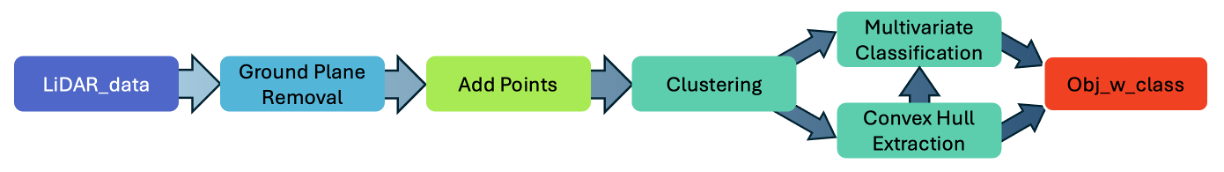
\includegraphics[width=0.95\linewidth]{Images/gbcache/gbcache_flow.png}
    \caption{Block diagram of GB-CACHE process flow.}
    \label{fig:gbcache_flow}
\end{figure}

Each segmented object is then identified by a concave hull formed from the $x$ and $y$ vertices of a perimeter-matched polygon.
Compared to axis-aligned bounding boxes or circular boundary approximations, concave hulls more accurately reflect object geometry without overgeneralizing the object’s spatial extent.

For autonomous navigation, concave hulls offer a balance between fidelity and operational safety.
This is especially relevant in ground-based and maritime environments, where the ability to navigate between closely spaced objects depends on accurately estimating navigable pathways.
Overly conservative bounds may exaggerate the extent of objects as viewed from the vessel.
With precise object boundaries known, they can be inflated to accommodate navigational safety while maintaining an accurate representation of the object's structure.

GB-CACHE employs a \acl{MGC} to specify what class of object it has identified. 
Much like other classification methods, it utilizes a list of detected features to distinguish one class from another.
Each of the ten features it observes is provided with a brief description in Table \ref{tab:gbcache_features}.
The magnitude of an object's observed individual features may change based on distance to the object or viewing angle, but their relative values still provide valuable information.

\begin{table}[htbp]
\centering
\begin{tabular}{lll}
\hline
\multicolumn{3}{c}{GB-CACHE: Object Classification Features}\\
\hline
\hline
\textbf{No.} & \textbf{Feature Type} & \textbf{Description} \\ 
\hline
1 & Intensity (Max) & Peak LiDAR return intensity \\
2 & Intensity (Min) & Lowest LiDAR return intensity \\
3 & Intensity (Avg) & Mean LiDAR return intensity \\
4 & Intensity (Std. Deviation) & Variation in return intensity \\
5 & Height (Max) & Vertical extent of the object \\
6 & Filled Cell Count & Number of occupied grid cells \\
7 & Polygon Perimeter & Length of 2D concave hull boundary \\
8 & Polygon Area & Area of enclosed 2D concave hull \\
9 & Major Axis Length & Longer principal axis of object polygon \\
10 & Minor Axis Length & Shorter principal axis of object polygon \\
\hline
\end{tabular}
\caption{Features used for GB-CACHE multivariate classification.}
\label{tab:gbcache_features}
\end{table}

In \ac{MGC}, the values of these features are assumed to follow Gaussian distributions within each class.
By modeling the joint distribution of all ten features at once (a multivariate Gaussian), the classifier can compute a \acl{PDF} for each object class.
This enables the classifier to assign the most probable class label to the object based on the vector of all ten features, even as the individual values may fluctuate.

% \begin{figure}
%     \centering
%     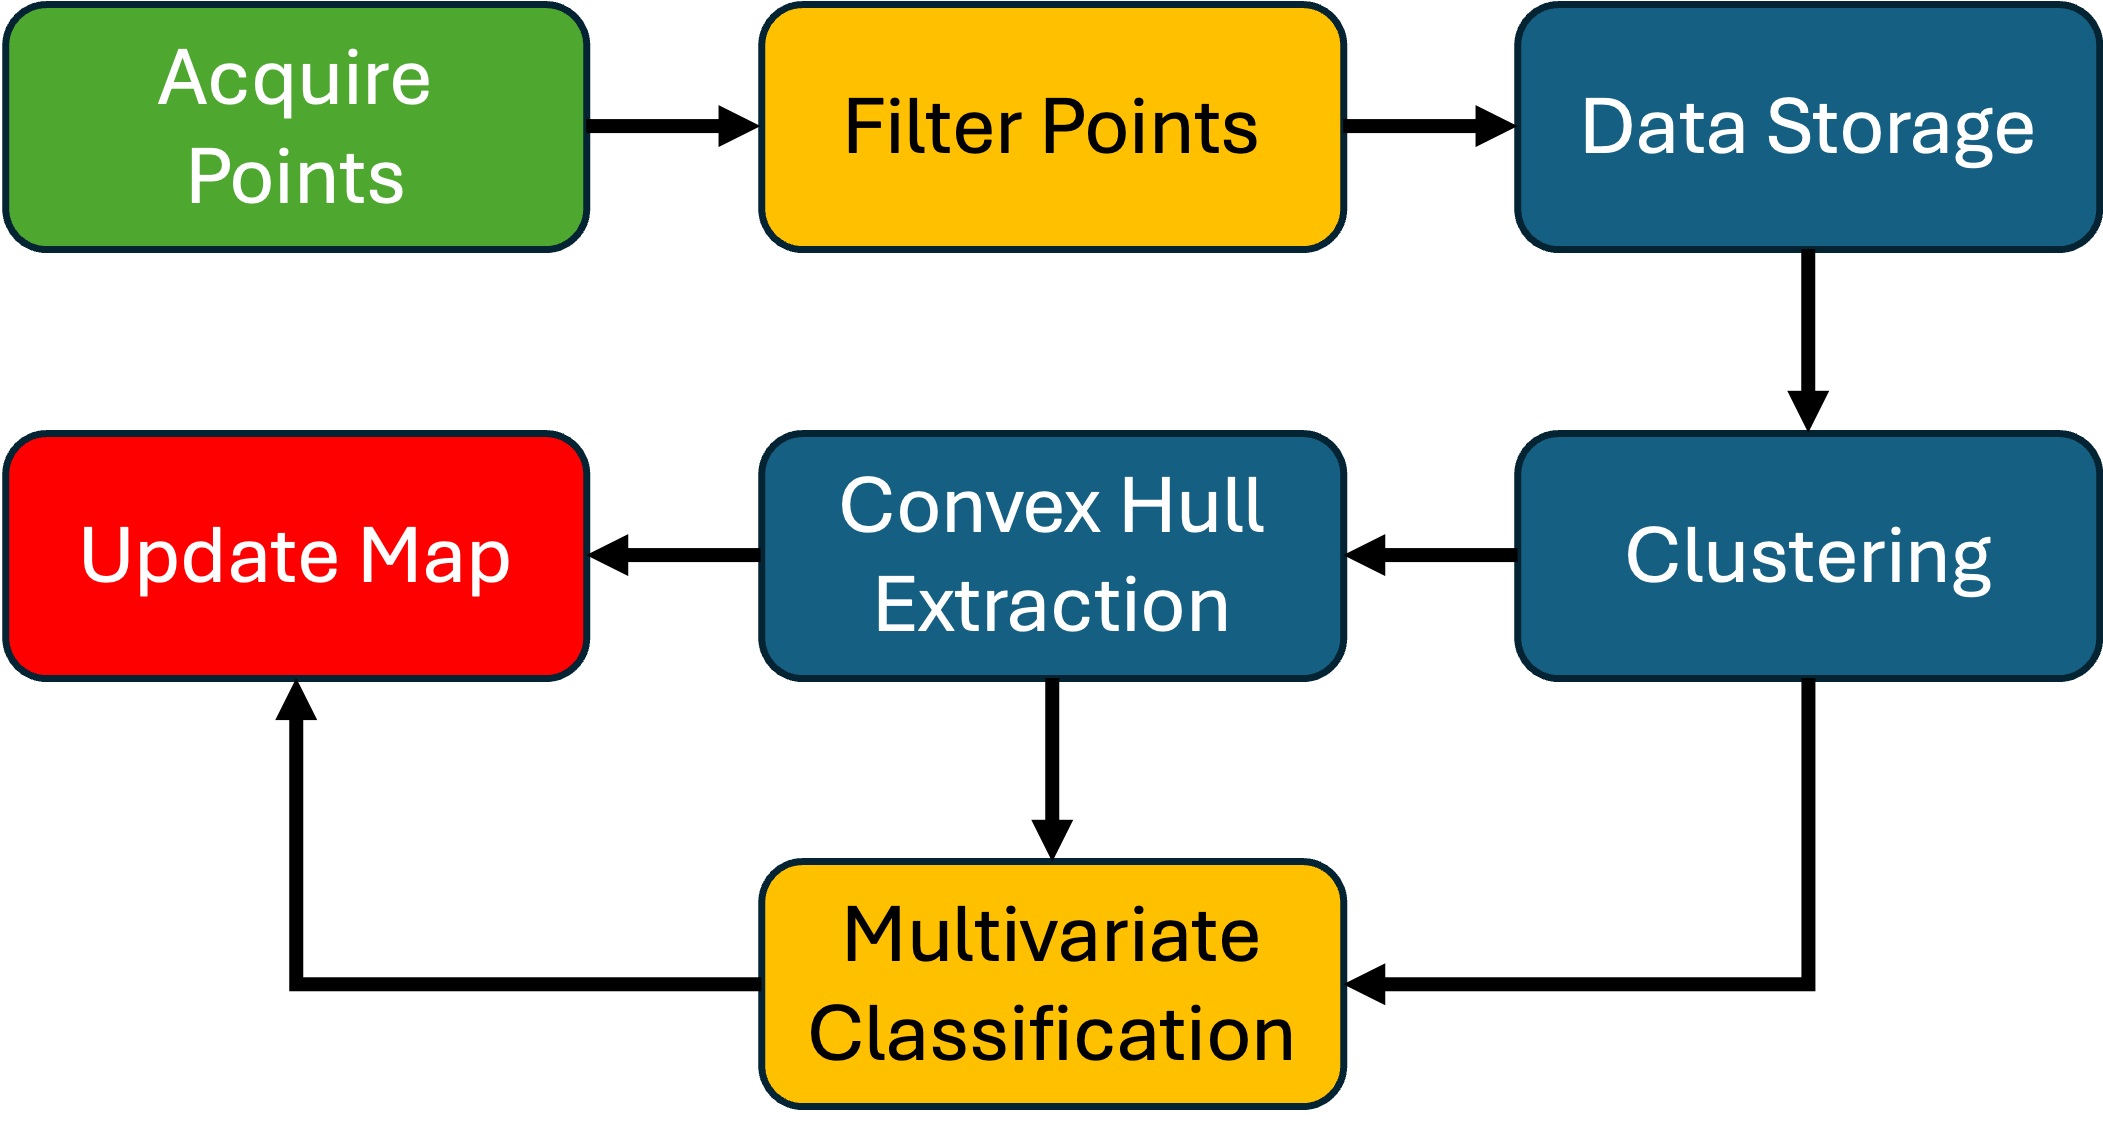
\includegraphics[width=0.95\linewidth]{Images/gbcache_flow.png}
%     \caption{Rectangular bounding boxes placed around maritime objects detected by a re-trained YOLO detection model.}
%     \label{fig:gbcache_flow}
% \end{figure}

% The YOLO Framework
% Describe the principle succinctly:

% YOLOv8 Architecture

% This section should flow from general framework to version-specific improvements:

% Image Resolution and Input Scaling
% Transition to operational detail and experimental consistency:

% Detection Scale and Spatial Sensitivity
% Discuss how feature maps relate to the detection limit:

% Model Constraints and Applicability
% Then note practical limitations and their relevance:

% Implications for Real-Time Fusion
% Conclude the section by connecting to your larger research goal:

% %%%%%%%%%%%%%%%%%%%%%%%%%%%%%%%%%%%%%%%%%%%%%%%%%%%%%%%%%%%%%%%%%%%%
% \subsection{Grid-Based Indexing} \label{sec:grid-based_indexing}

% Reliable object detection from LiDAR data is essential for safe maritime autonomy. To process large three-dimensional point clouds efficiently, this work applies the Grid-Based Clustering and Concave Hull Extraction (GB-CACHE) framework, an existing method developed for real-time segmentation of sparse LiDAR data. The approach enables rapid separation of individual objects while maintaining computational efficiency compatible with embedded vessel hardware.

% GB-CACHE operates by organizing each LiDAR scan into a structured spatial grid, allowing nearby points to be grouped without requiring full pairwise distance comparisons. This grid representation simplifies the process of identifying discrete clusters that correspond to physical objects such as buoys, vessels, or markers. By tuning grid size and connectivity thresholds, the method balances sensitivity to small targets against computational cost. In maritime environments—where LiDAR returns are sparse and concentrated on a few floating objects—the grid structure efficiently isolates relevant regions while ignoring the large volumes of empty space above and below the water surface.

% \begin{figure}
%     \centering
%     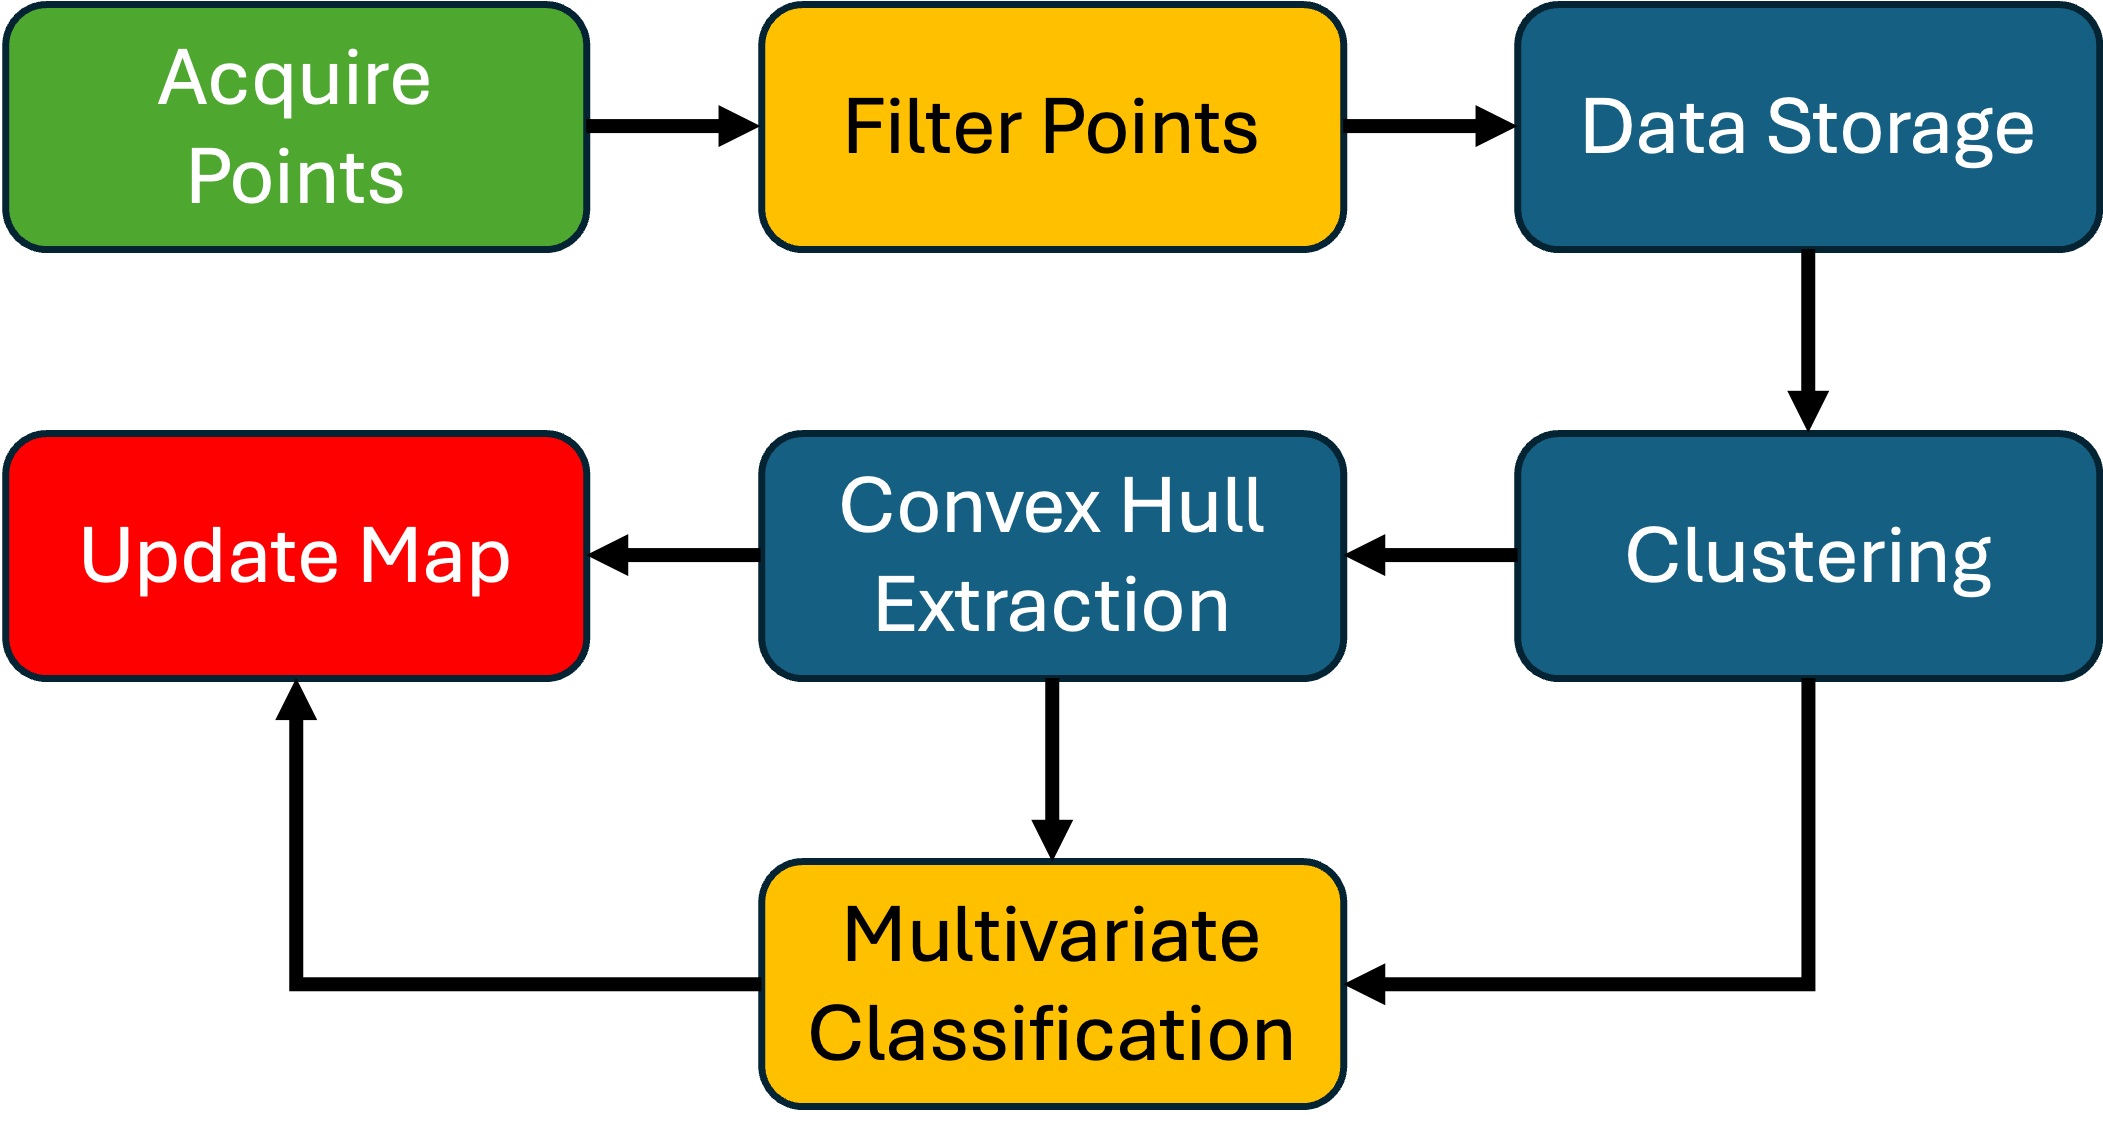
\includegraphics[width=0.5\linewidth]{Images/gbcache_flow.png}
%     \caption{Functional block diagram of the GB-CACHE workflow.}
%     \label{fig:gbcache_flow}
% \end{figure}

% Once potential objects are identified, GB-CACHE extracts geometric boundaries that define their overall shape. Each detected cluster is represented by a concave hull, which conforms closely to the true object outline rather than enclosing it with a simple convex boundary. This representation preserves important geometric details for irregular maritime targets, such as navigation buoys or vessel superstructures, while remaining compact for downstream processing. The resulting shape models form the basis for feature extraction and classification in subsequent stages of the perception pipeline.

% The algorithm’s design emphasizes computational efficiency and predictable timing. Grid-based indexing ensures that processing time scales linearly with the number of points in a scan, allowing consistent real-time performance. Each LiDAR frame is processed independently—populating the grid, segmenting occupied regions, and generating hulls—without maintaining historical state or iterative refinement. This stateless design simplifies implementation and guarantees bounded latency, which is critical for collision-avoidance and control tasks.

% GB-CACHE’s lightweight memory requirements further support real-time operation. Because memory usage scales with grid dimensions rather than total point count, resource consumption remains stable across varying environmental conditions. The method thus provides a practical and computationally efficient means of segmenting maritime LiDAR data into meaningful object candidates, serving as the front-end detection stage for the overall perception system.

% The segmentation stage of \ac{GB-CACHE} produces a structured list of clustered objects, each represented by a polygonal boundary and associated point statistics.
% The multivariate Gaussian classifier (MGC) operates in parallel to this process, classifying each object in the list based on geometric and intensity-derived features computed from its segmented point cloud.
% This architecture separates detection from classification, enabling each to be optimized and evaluated independently while maintaining real-time operation.

% For each detected object, a ten-dimensional feature vector is extracted that captures both spatial geometry and surface reflectivity characteristics.
% The geometric features describe object shape and scale, while the intensity-based features provide cues related to material properties and orientation of reflective surfaces.
% These complementary measurements form a compact yet discriminative representation suitable for statistical classification.
% The selected features are summarized in Table~\ref{tab:gbcache_features}.

% \begin{table}[htbp]
% \centering
% \begin{tabular}{lll}
% \hline
% \multicolumn{3}{c}{GB-CACHE: Object Classification Features}\\
% \hline
% \hline
% \textbf{No.} & \textbf{Feature Type} & \textbf{Description} \\ 
% \hline
% 1 & Maximum Intensity & Peak LiDAR return intensity \\
% 2 & Minimum Intensity & Lowest LiDAR return intensity \\
% 3 & Average Intensity & Mean LiDAR return intensity \\
% 4 & Intensity Standard Deviation & Variation in return intensity \\
% 5 & Maximum Height & Vertical extent of the object \\
% 6 & Filled Cell Count & Number of occupied grid cells \\
% 7 & Polygon Perimeter & Boundary length of concave hull \\
% 8 & Polygon Area & Enclosed area of concave hull \\
% 9 & 2D Minor Axis Length & Shorter principal axis of object shape \\
% 10 & 2D Major Axis Length & Longer principal axis of object shape \\
% \hline
% \end{tabular}
% \caption{Features used for GB-CACHE multivariate classification.}
% \label{tab:gbcache_features}
% \end{table}

% The MGC models the joint probability distribution of these features for each object class under the assumption of Gaussian statistics.
% Each class is represented by its mean vector and covariance matrix, estimated from labeled training data.
% During inference, the classifier computes the likelihood of an observed feature vector under each class model and assigns the class with the highest posterior probability.
% This probabilistic formulation captures correlations among features and yields confidence estimates that can be used downstream in fusion or decision logic.

% Feature-based classification offers several advantages for real-time maritime perception.
% It requires minimal training data, provides interpretability of the decision process, and imposes negligible computational overhead.
% Unlike deep-learning models that operate directly on raw point clouds, the MGC approach allows rapid retraining or adaptation to new object categories without altering the underlying clustering framework.
% This modularity supports continuous improvement and integration within the real-time perception pipeline illustrated in Figure~\ref{fig:gbcache_flow}.

% \begin{figure}[htbp]
%     \centering
%     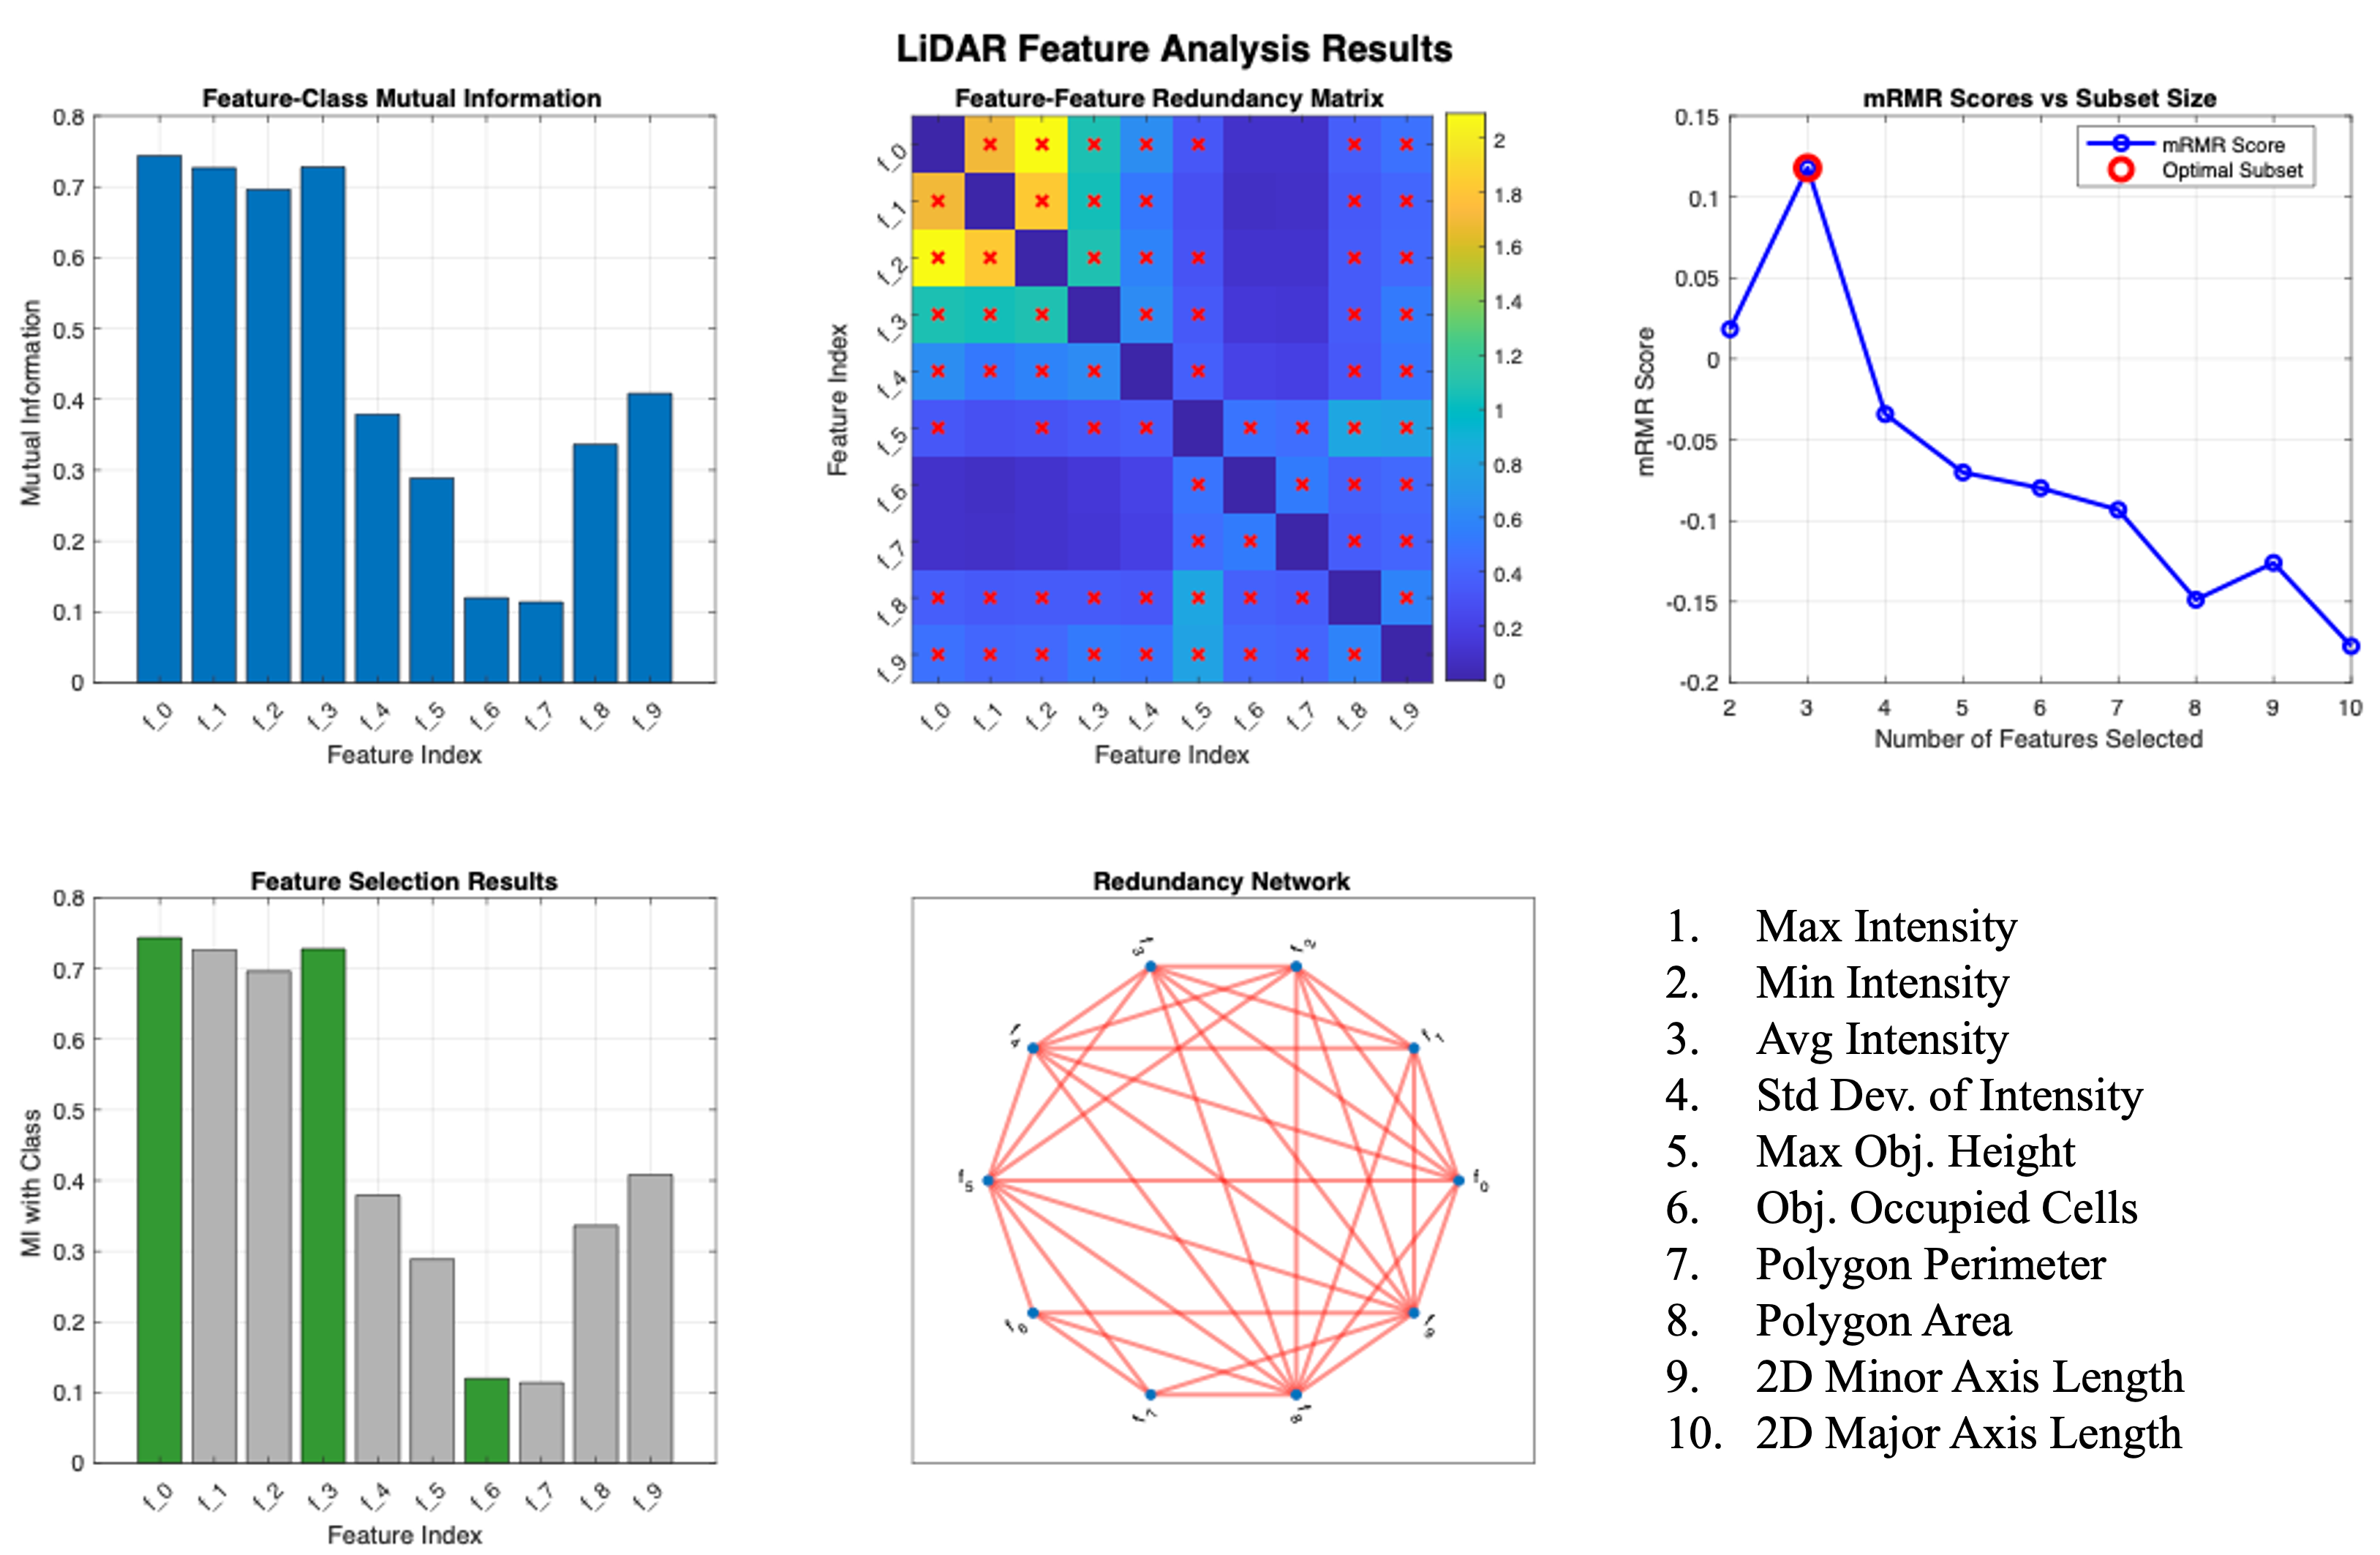
\includegraphics[width=0.95\linewidth]{Images/info_theory_chart_1.png}
%     \caption{Caption}
%     \label{fig:infoTheory_chartsA}
% \end{figure}

% \begin{figure}[htbp]
%     \centering
%     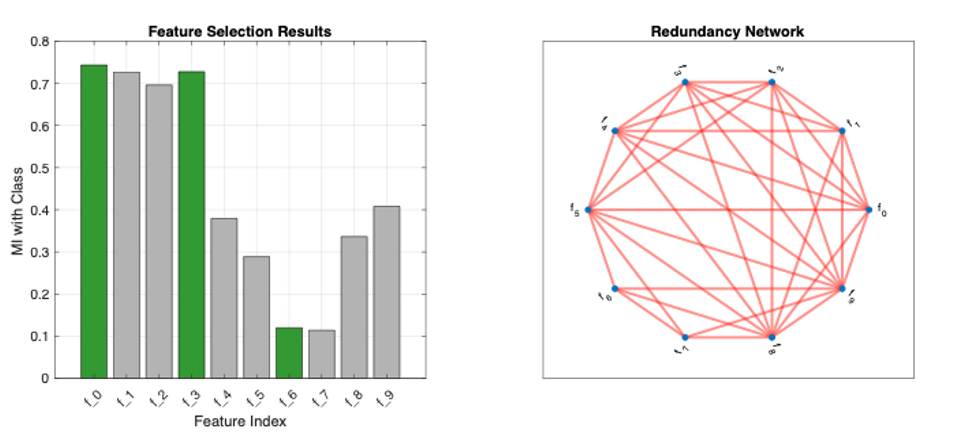
\includegraphics[width=0.8\linewidth]{Images/info_theory_chart_2.png}
%     \caption{Caption}
%     \label{fig:infoTheory_charts}
% \end{figure}



%%%%%%%%%%%%%%%%%%%%%%%%%%%%%%%%%%%%%%%%%%%%%%%%%%%%%%%%%%%%%%%%%%%%
%%%%%%%%%%%%%%%%%%%%%%%%%%%%%%%%%%%%%%%%%%%%%%%%%%%%%%%%%%%%%%%%%%%%

\end{document}
